\section{Architektur}
\begin{frame}
    \frametitle{Architektur}
    \begin{minipage}{0.48\textwidth}
        \begin{itemize}
            \item Programmiersprache: TypeScript
            \item Store Framework: Yjs
            \item Frontend Technologie: Vue.js
            \item Backend: Node.js
            \item Datenbank: MongoDB
            \item Middleware: Mosquitto
            \item Protokolle: Websockets und MQTT
        \end{itemize}
    \end{minipage}
    \hfill
    \begin{minipage}{0.45\textwidth}
        \begin{figure}
            \centering
            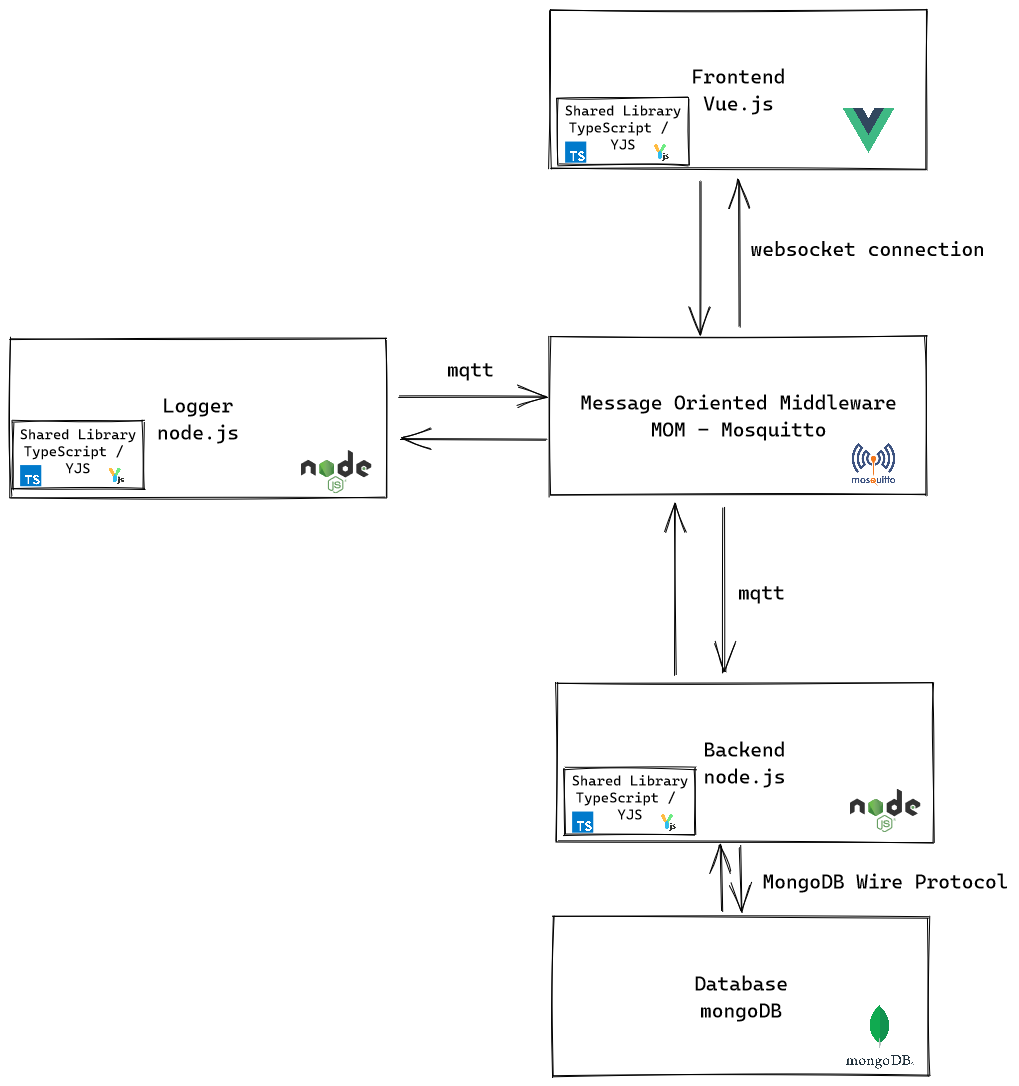
\includegraphics[height=6cm]{media/Big_Picture_wodss}
        \end{figure}
    \end{minipage}
\end{frame}
\begin{frame}
    \frametitle{Anpassungen seit der Midterm Präsentation}
    \begin{itemize}
        \item \textit{Synchronized Store} wurde vereinfacht: shadow und synchronized State wurden konsolidiert.
        \item Eine verteilte Mutex wurde implementiert.
        \item Eine synchronisierter Session Store wurde umgesetzt.
        \item Die Kommunikation über das Internet wurde mittels SSL abgesichert.
        \item Das Backend wurde hochverfügbar und gemacht.
        \item Eine externe Logging Komponente wurde umgesetzt.
        \item Persistierung des Document Store in einer MongoDB wurde eingerichtet.
    \end{itemize}
\end{frame}
